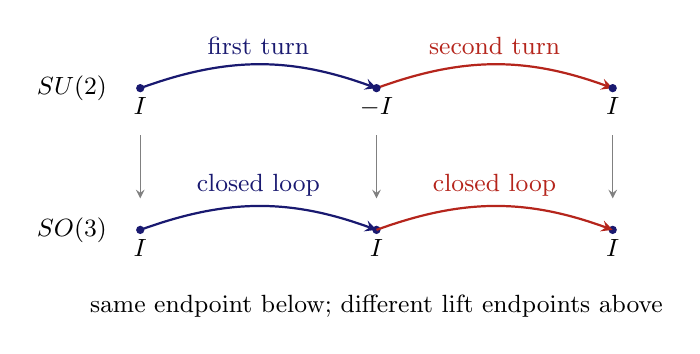
\begin{tikzpicture}[x=1cm,y=1cm,font=\small,>=stealth]
\node[left] at (-.3,1) {$SU(2)$};
\node[left] at (-.3,-.8) {$SO(3)$};
\coordinate (a) at (0,1);\coordinate (b) at (3,1);\coordinate (c) at (6,1);
\draw[->,MidnightBlue,thick] (a) to[bend left=20] node[above] {first turn} (b);
\draw[->,BrickRed,thick] (b) to[bend left=20] node[above] {second turn} (c);
\foreach \x/\lab in {0/I,3/-I,6/I}{
 \fill[MidnightBlue] (\x,1) circle (1.5pt);
 \node[below] at (\x,1) {$\lab$};
 \draw[gray,->] (\x,.4)--(\x,-.4);
 \fill[MidnightBlue] (\x,-.8) circle (1.5pt);
 \node[below] at (\x,-.8) {$I$};
}
\draw[->,MidnightBlue,thick] (0,-.8) to[bend left=20] node[above] {closed loop} (3,-.8);
\draw[->,BrickRed,thick] (3,-.8) to[bend left=20] node[above] {closed loop} (6,-.8);
\node[below] at (3,-1.5) {same endpoint below; different lift endpoints above};
\end{tikzpicture}
